\section{Sphinx Packet Format}
\label{sec:sphinx}

HOPR uses the Sphinx packet format \cite{sphinxpaper} to encapsulate and route data packets to their final recipient while achieving sender and recipient unlinkability. The Sphinx packet format determines how mixnet packets are created and transformed. This happens in a way that does not leak path information to relayers or other parties eavesdropping on the communication. A Sphinx packet consists of two parts, a header and an onion-encrypted payload:

\begin{figure}[H]
    \centering
    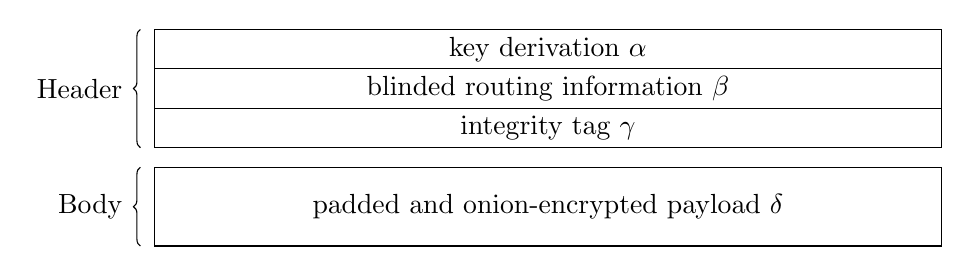
\begin{tikzpicture}
        \draw (0,0) rectangle (10,0.5);
        \draw (0,-0.5) rectangle (10,0);
        \draw (0,-1) rectangle (10,-0.5);

        \draw (5,0.25) node {key derivation $\alpha$};
        \draw (5,-0.25) node {blinded routing information $\beta$};
        \draw (5,-0.75) node {integrity tag $\gamma$};

        \draw[decoration={brace,raise=5pt,mirror},decorate] (0,0.5) -- node[left=8pt] {Header} (0,-1);

        \draw (0,-2.25) rectangle (10, -1.25);
        \draw (5,-1.75) node {padded and onion-encrypted payload  $\delta$};

        \draw[decoration={brace,raise=5pt,mirror},decorate] (0,-1.25) -- node[left=8pt] {Body} (0,-2.25);
    \end{tikzpicture}
    \label{fig:sphinxoverview}
    \caption{Schematic overview of a SPHINX packet}
\end{figure}

\subsection{Construction}

The following explains how a Sphinx packet is created and how it is transformed at each hop before arriving at its final destination. First, the sender chooses a path (see Section \ref{sec:path-selection}), and derives shared keys with each node on the path. The shared keys serve as a master secret to derive subkeys. These subkeys are used to blind the routing information in such a way that nodes can solely determine the next downstream node, and also to create an authentication tag to check the integrity of the header. In addition, the sender applies one layer of encryption for each node along the chosen path to the payload. This accomplished, the sender finally sends the packet to the first hop.

Once a node receives a mixnet packet, it first derives the key that it has shared with the sender of the packet and checks the integrity of the header. Next, it unblinds the routing information to determine the next downstream node and removes one layer of encryption from the encrypted payload. At this point, the node is able to decide whether it is the final recipient of the message or it is supposed to forward the packet to the next hop.\footnote{TODO: Make explicit the conditions behind this decision.}

\begin{comment}
\paragraph{Notation:}Let $\kappa=128$ be the security parameter. With non-negligible probability, an adversary must perform around $2^\kappa$ operations to break the security of Sphinx.

Let $r$ be the maximum number of nodes that a Sphinx mix message will traverse before being delivered to its destination.

$G$ is a prime order cyclic group satisfying the decisional Diffie-Hellman assumption \cite{Boneh_1998}. We use the secp256k1 elliptic curve \cite{secp}. The element $g$ is a generator of $G$ and $q$ is the (prime) order of $G$, with $q\approx2^{2*\kappa}$.

$G^*$ is the set of non-identity elements of G. $h_b$ is a pre-image resistant hash function used to compute blinding factors and modelled as a random oracle such that
$h_b:G^*\times G^*\rightarrow\mathbb{Z}^*_q$, where $\mathbb{Z}^*_q$ is the field of non-identity elements of $\mathbb{Z}_q$ (field of integers). We use the BLAKE2s hash function \cite{blake2}.

Each node $i$ has a private key $x_{i}\in \mathbb{Z}^*_q$ and a public key $y_{i}=g^{x_{i}}\in G^*$.
$\alpha_i$ is the group elements which, when combined with the nodes’ public keys, allow a shared key to be computed for each via Diffie-Hellman (DH) key exchange. This ensures that each node in the user-chosen route can forward the packet to the next, and only the receiving mix node can decrypt it.
$s_i$ are the DH shared secrets, $b_i$ are the blinding factors.
\end{comment}

\subsubsection{Key Extraction}
\label{sec:sphinx:keyderivation}

Path selection (see Section \ref{sec:path-selection}), results in a list $n_0, \dots, n_r$ of mix nodes which are supposed to process and forward the packet before the packet reaches its destination $dest$. HOPR nodes use their public keys as addresses, hence the public keys $Y_0, \dots , Y_r$ are known to the creator of a packet.\footnote{TODO: Make this more explicit in section \ref{sec:path-selection}.}

\paragraph{Key Exchange}

Having this knowledge allows the creator of the packet to perform an offline Diffie-Hellman key exchange with each of the mix nodes $n_0 , \dots , n_r$ and the destination $dest$, resulting in shared secrets $s_0, \dots , s_r$, and $s_{dest}$.

To provide perfect forward secrecy and thereby minimize the risk of key corruption, the sender first samples a random value $x \in \mathbb{F}$ and derives $\alpha_0 = x \cdot G$.\footnote{TODO: Properly introduce $G$} It further derives blinding factor $b_0$ as $b_0 = \mathsf{KDF}(\alpha_0, x \cdot Y_0)$ where $\mathsf{KDF}(salt, secret)$ is a key derivation function (see Appendix \ref{appendix:keyderivation}), and derives the shared secret as $s_0 = x \cdot b_0 \cdot Y_0$. Hence, deriving the shared secret $s_0$ requires knowledge of the sender's field element $\alpha_0 = x \cdot G$ as well as the receivers' field element $x \cdot b_0 \cdot Y_0$.

The first relayer $n_0$ is then able to compute $s_0$ by first deriving $x \cdot Y_0$ as

$$y_0 \cdot \alpha_0 = y_0 \cdot x \cdot G = x \cdot ( y_0 \cdot G) = x \cdot Y_0$$

yielding $b_0$ and $s_0 = y_0 \cdot b_0 \cdot \alpha_0$ where $y_0$ refers to the private key of node $n_0$. The value $s_0$ then servers as a master secret to perform further key derivations as described in Appendix \ref{appendix:keyderivation}.

\paragraph{Transformation}

Once the key extraction is complete, the each relayer $n_i$ transforms its value $\alpha_i$ into $\alpha_{i+1}$ by setting $\alpha_{i+1} = b_i \cdot \alpha_i$ such that

$$ \alpha_i = x \cdot \biggl(\prod_{j=0}^{i} b_j \biggr) \cdot G = \biggl(\prod_{j=0}^{i} b_j \biggr) \cdot \alpha_0 = \biggl(\prod_{j=k+1}^{i} b_j \biggr) \cdot \alpha_k $$

By adding an additional blinding for every node along the selected path, each incoming $\alpha_i$ and each outgoing $\alpha_{i+1}$ become indistinguishable from random numbers of the same length. Hence, an adversary who observes incoming and outgoing packets cannot use $\alpha$ to track packets.

Since each $s_{i+1}$ depends on $b_{i+1}$ and therefore on all $\alpha_0, \dots , \alpha_i$, the key extraction can only be done in the preset order; first derive $s_0$, then derive $s_1$ etc. Hence, an adversary is unable to extract keys in a more favourable order, e.g., because it has managed to compromise some but not all nodes on the path.

\paragraph{Example}

The following example shows the key extraction process for a sender $A$, three mix nodes $B, C, D$ and a receiver $Z$.

\begin{align*}
    (\alpha_B,b_B,s_B) & = (x \cdot G,\textsf{KDF}(\alpha_B, y_B \cdot \alpha_B), y_B \cdot \alpha_B )                   \\
    (\alpha_C,b_C,s_C) & = (x \cdot b_B \cdot G,\textsf{KDF}(\alpha_C, y_C \cdot \alpha_C), y_C \cdot \alpha_C )             \\
    (\alpha_D,b_D,s_D) & = (x \cdot b_B \ b_C \cdot G,\textsf{KDF}(\alpha_D, y_D \cdot \alpha_D), y_D \cdot \alpha_D )       \\
    (\alpha_Z,b_Z,s_Z) & = (x \cdot b_B \ b_C \ b_D \cdot G,\textsf{KDF}(\alpha_Z, y_Z \cdot \alpha_Z), y_Z \cdot \alpha_Z ) \\
\end{align*}

where $y_i$ for $i \in \{ B,C,D,Z \}$ refers to the nodes' private keys and $s_i$ denotes the derived shared secret group elements.

Packets consist of $(\alpha, \beta, \gamma)$ where $\beta$ is described in section \ref{sec:sphinx:routinginformation} and $\gamma$ in section \ref{sec:sphinx:integrity}, leaving both underspecified for the moment. Further, let $packet_i = (\alpha_i, \beta_i, \gamma_i)$, leading to:

\begin{figure}[H]
    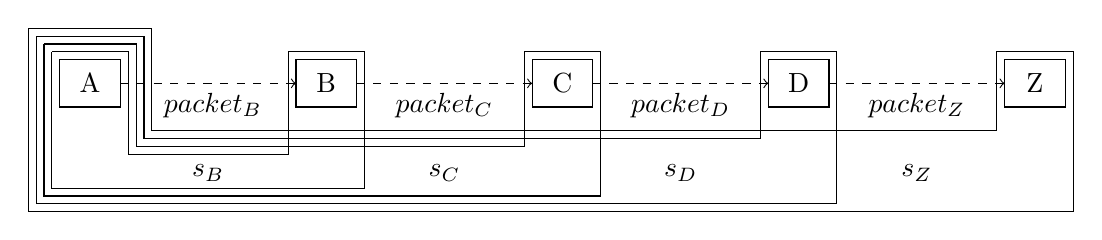
\begin{tikzpicture}
        \def\offset{3}
        \def\nodeWidth{0.77}
        \def\padding{0.93}
        \def\lowerpadding{0.7}
        \def\nodeHeight{0.6}
        \foreach \i\name\bi\packetName in{0/A/0/$packet_A$,1/B/$b_B$/$\ packet_B$,2/C/${b_C}$/$packet_C$,3/D/$b_D$/$packet_D$,4/Z/$b_Z$/$packet_Z$} {
                \draw (\i*\offset,0) rectangle (\i*\offset+\nodeWidth,\nodeHeight) node [midway] {\name};

                \ifnum\i>0
                    \draw (-0.1*\i,\nodeHeight+0.1*\i) -- (-0.1*\i,-\padding-0.1*\i) -- (\i*\offset+0.1+\nodeWidth,-\padding-0.1*\i) -- (\i*\offset+0.1+\nodeWidth,\nodeHeight+0.1) -- (\i*\offset-0.1,\nodeHeight+0.1) -- (\i*\offset-0.1,-\lowerpadding+0.1*\i) -- (\nodeWidth+0.1*\i,-\lowerpadding+0.1*\i) -- (\nodeWidth+0.1*\i,\nodeHeight+0.1*\i) -- (-0.1*\i,\nodeHeight+0.1*\i);
                \fi

                \ifnum\i>0
                    \draw [->,dashed] (\i*\offset-\offset+\nodeWidth,0.3) -- (\i*\offset,0.3) node [midway,below] {\packetName} node [midway,below=26pt] {{\smaller$s_{\name}$}};
                \fi
            }
    \end{tikzpicture}
    \caption{Node $A$ derives shared keys $s_B, s_C, s_D, s_Z$ with node $B, C, D, Z$ using their public keys $Y_B, Y_C, Y_D, Y_Z$.}
    \label{fig:sphinx:keyderivation}
\end{figure}

\subsubsection{Replay protection}
\label{sec:sphinx:replayprotection}

The creator of a packet picks a path that the packet is supposed to take. As seen in section \ref{sec:sphinx:keyderivation}, the key derivation is done such that the packet cannot be processed in a order than the one chosen by its creator.

This behavior prevents the adversary from changing the route but also allows no other route. Hence the adversary can be sure that there is no second possible route. Therefore, it can try to replicate the packet and send it multiple to see which connections get used more and thus reveals the route of the packet.

To prevent from this attack scenario, each node $n_i$ computes a fingerprint $s_i^{tag}$ of each processed packet and stores it in order to refuse the processing of already seen packets. The value $s_i^{tag}$ is generated from master secret $s_i$ as seen in section \ref{sec:sphinx:keyderivation} using the key derivation described in section \ref{appendix:keyderivation}.

\subsubsection{Routing information}
\label{sec:sphinx:routinginformation}

Each node on the path needs to decide whether it is destined to be the receiver of the message and if not, to whom it is supposed to forward the packet. To achieve the privacy properties, each node must only know its direct successor and is allowed to know its predecessor. More precisely, the node must not be able to determine \textit{if} and \textit{where} the next downstream node is going to forward the packet to. Nor shall it know where the packet came from before it was sent to its predecessor.

This is achieved by applying multiple layers of blinding and sequentially removing layer by layer at each hop such that the address of the next hop is only visible for one hop along the path.

To ensure that the header has not been tampered while traveling through and network and being transformed by the nodes along the path, there is an integrity tag that is sent in addition to the public key of the next hop. The routing information is thus given by $(y_i, \gamma_i)$ where $y_i$ denotes the public key and $\gamma_i$ the integrity tag for the next downstream node. See section \ref{sec:sphinx:integrity} for more details on the utilized integrity scheme.

\paragraph{Adresses}

Nodes in the network are distinguished by the ECDSA public keys, hence the header includes the public key of the next downstream node and in case of the very last node, a distinguished byte sequence $END$.

ECDSA public keys are given by tuple of two 32-byte field elements $(x,y)$, upon which it is sufficient to solely store the first component $x$ and the sign of $y$, resulting in a \textsf{compressed} elliptic curve point \textsf{0x02}\textless\textsf{x}\textgreater{} for positive $y$ and \textsf{0x03}\textless\textsf{x}\textgreater{} otherwise. The sequence $END$ is given as \textsf{0x04} such that the last node can ignore all subsequent bytes if $END$ is present.

\paragraph{Blinding}

The header uses multiple blindings and their aggregations to make certain sections of the header visible to only a single node. Blindings are generated by a pseudorandomness generator (PRG), see appendix \ref{appendix:prg} for a detailed description of the utilized PRG.

As a result of the Diffie-Helman key exchange done in section \ref{sec:sphinx:keyderivation}, each node along the path is able to derive a shared secret $s_i$ with the creator of the packet and is therefore able to derive a sub-key $s_i^{bl}$. Both, creator of the packet and each node $n_i$ along the path use $s_i^{bl}$ as a seed for the PRG, yielding $blinding_i$.

The routing information for each node $n_i$ is blinded by XORing the content with $blinding_i$ as well as the blindings $blinding_0, \dots , blinding_{i-1}$ of all previous hops. Each node that receives the packet, removes their own blinding from the header and is thus able to extract the routing information destined for them. By removing the blinding from the header, it allows the next downstream node to extract their routing information since it is now only blinded by their blinding.

\paragraph{Example}

The following assumes the sender $A$ is generating routing information for $B,C,D,Z$ and applies their corresponding blinding before sending the header to the first relayer $B$. The blindings are visualized by different hatchings.

\begin{figure}[H]
    \centering
    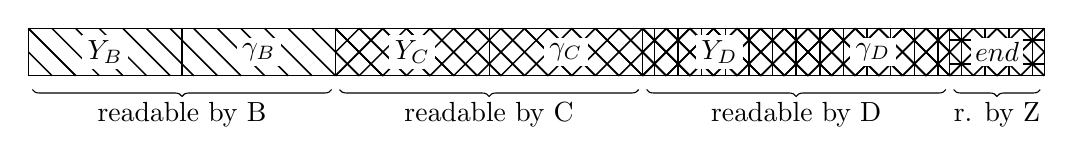
\begin{tikzpicture}
        \def\one{0.6}
        \def\scale{0.9}
        \def\nodeWidth{1.95}
        \def\endWidth{1.2}
        \def\width{3*2*\nodeWidth+\endWidth}
        \foreach \i\name in{0/B,1/C,2/D,3/Z} {
                \begin{scope}[shift={(\i*\nodeWidth*2,0)}]
                    \ifnum\i=0
                        \def\a{11.7}
                        \def\diff{11.1}
                    \fi

                    \ifnum\i=1
                        \def\a{7.8}
                        \def\diff{7.2}
                    \fi

                    \ifnum\i=2
                        \def\a{3.9}
                        \def\diff{3.3}

                    \fi

                    \ifnum\i=3
                        \def\a{\endWidth}
                        \def\diff{0.6}
                    \fi


                    \def\b{\one}
                    \def\lw{0.2}

                    \foreach \x [count=\i] in{0,0.3,0.6,...,\b}{
                            \draw [line width=\lw mm](\x,0)--(0,\x) (\a-\b+\x,\b)--(\a,\x);
                        }
                    \foreach \x [count=\i] in{0,0.3,0.6,...,\diff}{
                            \draw [line width=\lw mm](\x+\b,0)--(\x,\b);
                        }

                    \ifnum\i>0
                        \foreach \x [count=\i] in{0,0.3,0.6,...,\b}{
                                \draw [line width=\lw mm](0,\x)--(\b-\x,\b) (\a-\b+\x,0)--(\a,\b-\x);
                            }
                        \foreach \x [count=\i] in{0,0.3,0.6,...,\diff}{
                                \draw [line width=\lw mm](\x,0)--(\b+\x,\b);
                            }
                    \fi

                    \ifnum\i>1
                        \foreach \x [count=\i] in{0.15,0.45,...,\a}{
                                \draw [line width=\lw mm](\x,0)--(\x,\b);
                            }
                    \fi

                    \ifnum\i>2
                        \foreach \x [count=\i] in{0.15,0.45,...,\b}{
                                \draw [line width=\lw mm](0,\x)--(\a,\x);
                            }
                    \fi
                \end{scope}
                \ifnum\i<3
                    \draw [color=white] (\i*2*\nodeWidth,0) rectangle (\i*2*\nodeWidth+\nodeWidth,\one) node [midway,color=black,fill=white,inner sep=2pt] {$Y_{\name}$};
                    \draw (\i*2*\nodeWidth,0) -- (\i*2*\nodeWidth,\one);
                    \draw [color=white] (\i*2*\nodeWidth+\nodeWidth,0) rectangle (\i*2*\nodeWidth+2*\nodeWidth,\one) node [midway,color=black,fill=white,inner sep=2pt] {$\gamma_{\name}$};
                    \draw (\i*2*\nodeWidth+\nodeWidth,0) -- (\i*2*\nodeWidth+\nodeWidth,\one);

                    \draw[decoration={brace,raise=5pt,mirror},decorate] (\nodeWidth*2*\i+0.05,0) -- (\nodeWidth*2*\i+\nodeWidth*2-0.05,0) node[midway,below=6pt] {readable by \name};
                \else
                    \draw [color=white] (\i*2*\nodeWidth,0) rectangle (\i*2*\nodeWidth+\endWidth,\one) node [midway,color=black,fill=white,inner sep=1.5pt] {$end$};
                    \draw (\i*2*\nodeWidth,0) -- (\i*2*\nodeWidth,\one);

                    \draw[decoration={brace,raise=5pt,mirror},decorate] (\i*2*\nodeWidth+0.05,0) -- (\i*2*\nodeWidth+\endWidth-0.05,0) node[midway,below=6pt] {r. by \name};
                \fi
            }

        \draw (0,0) rectangle (\width,\one);
    \end{tikzpicture}
    \caption{Blinded routing information sent to first relayer $B$.}
\end{figure}
\subsubsection{Delete and shift}
\label{sec:sphinx:shifting}

Unblinding the $\beta_i$ reveals the public key $Y_{i+1}$ of the next downstream node as well as the integrity tag $\gamma_{i+1}$ that allows the next downstream to verify the integrity of $\beta_{i+1}$. The $rest$ of $\beta_i$ is kept hidden to the node as it contains random data, see section \lcnameref{sec:sphinx:shorterpaths}, \textit{or} blindings from other nodes which is assumed to be indistinguishable by that node.\footnote{TODO: Add brief explanation and/or reference for this assumption}

$$ \{ Y_{i+1}, \gamma_{i+1}, rest \} = \beta_i \oplus \textsf{PRG}_{s_i^{bl}}(0, | \beta |) $$

After extracting $Y_{i+1}$ and $\gamma_{i+1}$, the node shifts $rest$ to the beginning and thereby overwrites its own routing information $Y_{i+1}$ and $\gamma_{i+1}$. In addition, it fills the hole in the end by adding its own blinding:

$$ \beta_{i+1} = rest \ || \ \textsf{PRG}_{s_i^{bl}}(| \beta |, | \beta | + |Y| + |\gamma|)$$

Note that the blindings are created using different boundaries. The first blinding is created from 0 to length of $\beta$ and the second one is created as if public key and integrity were appended in the end of $\beta$, hence boundaries are set from $| \beta |$ to $| \beta | + |y| + |\gamma|$.

\begin{figure}[H]
    \centering
    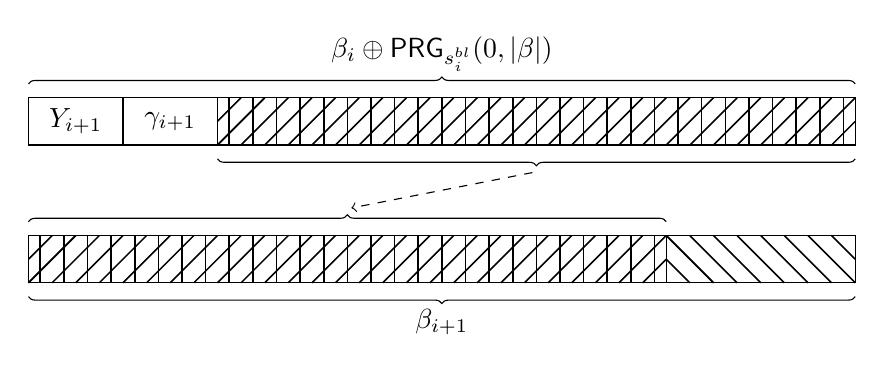
\begin{tikzpicture}
        \def\betaLength{10.5}
        \def\pubKey{1.2}
        \def\authTag{1.2}
        \def\one{0.6}

        \foreach \i in{0,1} {
                \begin{scope}[shift={(0,-1.75*\i)}]
                    \draw (0,0) rectangle (\betaLength,\one);

                    \ifnum\i=0
                        \def\shift{\pubKey+\authTag}
                        \draw (0,0) rectangle (\pubKey,\one) node[midway] {$Y_{i+1}$};
                        \draw (\pubKey,0) rectangle (\pubKey+\authTag,\one) node[midway] {$\gamma_{i+1}$};

                        \draw[decoration={brace,raise=5pt},decorate] (0,\one) -- (\betaLength,\one) node [midway,above=6pt] {$\beta_i \oplus \textsf{PRG}_{s_i^{bl}}(0, | \beta |)$};
                        \draw[decoration={brace,raise=5pt,mirror},decorate] (\authTag+\pubKey,0) -- (\betaLength,0);
                    \else
                        \def\shift{0}
                        \begin{scope}[shift={(\betaLength-\pubKey-\authTag,0)}]
                            \def\a{2.4}
                            \def\b{0.6}
                            \def\lw{0.2}
                            \def\diff{1.8}
                            \foreach \x [count=\i] in{0,0.3,0.6,...,\b}{
                                    \draw [line width=\lw mm](\x,0)--(0,\x) (\a-\b+\x,\b)--(\a,\x);
                                }
                            \foreach \x [count=\i] in{0,0.3,0.6,...,\diff}{
                                    \draw [line width=\lw mm](\x+\b,0)--(\x,\b);
                                }
                            \draw (0,0) -- (0,\one);
                        \end{scope}
                        \draw[decoration={brace,raise=5pt},decorate] (0,\one) -- (\betaLength-\authTag-\pubKey,\one);
                        \draw[decoration={brace,raise=5pt,mirror},decorate] (0,0) -- (\betaLength,0) node [midway,below=6pt] {$\beta_{i+1}$};
                    \fi

                    \begin{scope}[shift={(\shift,0)}]
                        \def\a{8.1}
                        \def\b{\one}
                        \def\lw{0.2}
                        \def\diff{7.5}

                        \foreach \x [count=\i] in{0,0.3,0.6,...,\b}{
                                \draw [line width=\lw mm](0,\x)--(\b-\x,\b) (\a-\b+\x,0)--(\a,\b-\x);
                            }
                        \foreach \x [count=\i] in{0,0.3,0.6,...,\diff}{
                                \draw [line width=\lw mm](\x,0)--(\b+\x,\b);
                            }

                        \foreach \x [count=\i] in{0,0.15,0.45,...,\a}{
                                \draw [line width=\lw mm](\x,0)--(\x,\b);
                            }
                    \end{scope}
                \end{scope}
            }

        \def\halfBeta{{(\betaLength-\pubKey-\authTag)}*0.5}
        \draw [->,dashed] (4.0+\pubKey+\authTag, -0.35) -- (4.1, -0.8);
    \end{tikzpicture}
    \caption{Shifting in the header}
\end{figure}
\subsubsection{Integrity check}
\label{sec:sphinx:integrity}

Upon reception of a packet, each node first derives the shared key $s_i$ with the creator of the packet. Before it unblinds the routing information, it checks their integrity and \textit{should} drop the packet if the header has been tampered.

\paragraph{Integrity tag}

As by section \ref{sec:sphinx:keyderivation}, each node along the path shares a secret $s_i$ with the creator of the packet. To create an integrity tag $\gamma_i$, the node first derives a sub-key $s_i^{int}$ as described in appendix \ref{appendix:keyderivation}, yielding:

$$\gamma_i = HMAC_{s_i^{int}}(\beta_i)$$

where $HMAC$ is instantiated with the hash function \textsf{BLAKE2s} and the output size is set to 32 bytes.

\paragraph{Packet transformation}

From the predecessor, which can be the creator of the packet \textit{or} a relayer, the node receives $\gamma_i$ and uses it to verify the integrity of the received header by recomputing the integrity tag $\gamma_i'$ using the received $\beta_i$ as well as the derived sub-key $s_i^{int}$ and checking whether $\gamma_i = \gamma_i'$. If this is not the case, the node drops the packet.

The node then applies the transformations from sections \ref{sec:sphinx:routinginformation} and \ref{sec:sphinx:shifting}, and thus receives not only the public key $y_{i+1}$ but also the integrity tag that the next downstream node needs to verify the integrity of the packet header.

\begin{figure}[H]
    \centering
    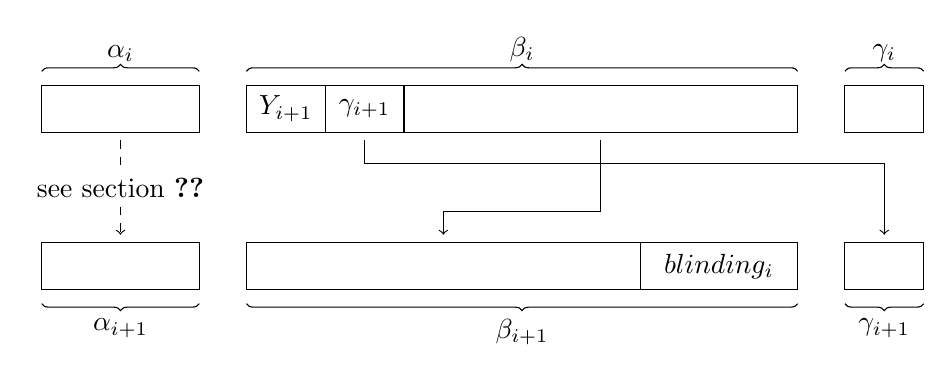
\begin{tikzpicture}
        \def\one{0.6}
        \def\alphaLength{2.0}
        \def\betaLength{7.0}
        \def\betaOffset{1.0}
        \def\gammaLength{1.0}
        \def\padding{0.6}
        \def\secondPacket{-2}

        \foreach \offset\i in{0/0,\secondPacket/1} {
                \begin{scope}[shift={(0,\offset)}]
                    \ifnum\i=0
                        \draw[decoration={brace,raise=5pt},decorate] (0,\one) -- node[above=5pt] {$\alpha_{i}$} (\alphaLength,\one);
                        \draw[->,dashed] (\alphaLength*0.5,-0.1) -- (\alphaLength*0.5,\secondPacket+\one+0.1) node [midway,fill=white] {see section \ref{sec:sphinx:keyderivation}};
                    \else
                        \draw[decoration={brace,raise=5pt,mirror},decorate] (0,0) -- node[below=7pt] {$\alpha_{i+1}$} (\alphaLength,0);
                    \fi
                    \draw (0,0) rectangle (\alphaLength,\one);

                    \begin{scope}[shift={(\alphaLength+\padding,0)}]
                        \ifnum\i=0
                            \draw[decoration={brace,raise=5pt},decorate] (0,\one) -- node[above=5pt] {$\beta_{i}$} (\betaLength,\one);
                            \draw (0,0) rectangle (\betaOffset,\one) node [midway] {$Y_{i+1}$};
                            \draw (\betaOffset,0) rectangle (\betaOffset+\betaOffset,\one) node [midway] {$\gamma_{i+1}$};

                            \draw[->] (\betaOffset+\betaOffset*0.5,-0.1) -- (\betaOffset+\betaOffset*0.5,-0.4) -- (\padding+\betaLength+\gammaLength*0.5,\secondPacket+\one+0.1+0.9) -- (\padding+\betaLength+\gammaLength*0.5,\secondPacket+\one+0.1);

                            \draw[->] (\betaOffset+\betaLength*0.5,-0.1) -- (\betaOffset+\betaLength*0.5,-0.1-0.9) -- (\betaLength*0.5-\betaOffset,-0.1-0.9) -- (\betaLength*0.5-\betaOffset,\secondPacket+\one+0.1);
                        \else
                            \draw[decoration={brace,raise=5pt,mirror},decorate] (0,0) -- node[below=7pt] {$\beta_{i+1}$} (\betaLength,0);
                            \draw (\betaLength-\betaOffset-\betaOffset,0) rectangle (\betaLength,\one) node [midway] {$blinding_i$};
                            \draw (\betaLength-2*\betaOffset,0) -- (\betaLength-2*\betaOffset,\one);
                        \fi


                        \draw (0,0) rectangle (\betaLength,\one);
                    \end{scope}

                    \begin{scope}[shift={(\alphaLength+\padding+\betaLength+\padding,0)}]
                        \ifnum\i=0
                            \draw[decoration={brace,raise=5pt},decorate] (0,\one) -- node[above=5pt] {$\gamma_{i}$} (\gammaLength,\one);
                        \else
                            \draw[decoration={brace,raise=5pt,mirror},decorate] (0,0) -- node[below=7pt] {$\gamma_{i+1}$} (\gammaLength,0);
                        \fi
                        \draw (0,0) rectangle (\gammaLength,\one);
                    \end{scope}
                \end{scope}
            }

    \end{tikzpicture}
    \caption{Extraction of $\gamma_{i+1}$ and creation of the next packet}
\end{figure}

The received header $(\alpha_i,\beta_i,\gamma_i)$ thereby transforms into $(\alpha_{i+1},\beta_{i+1},\gamma_{i+1})$.

\paragraph{Filler}

In order to compute the integrity tag, the sender needs to know \textit{how} the packet is going to look like when it reaches the node that checks its integrity. Hence, the creator of the packet needs to perform the whole transformations that are done by the relayers along the path \textit{in advance} before sending the packet.

\begin{figure}[H]
    \centering
    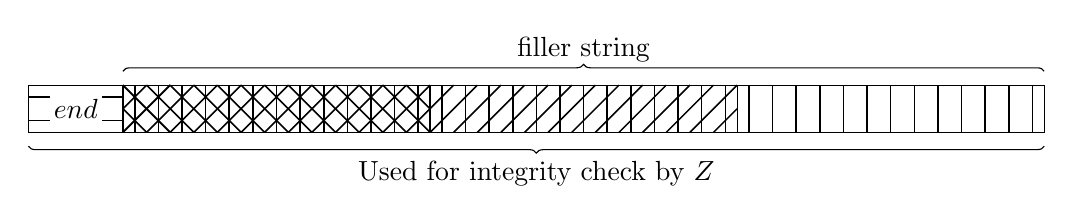
\begin{tikzpicture}
        \def\one{0.6}
        \def\scale{0.9}
        \def\nodeWidth{1.95}
        \def\endWidth{1.2}
        \def\width{3*2*\nodeWidth+\endWidth}
        \foreach \i\name in{0/B,1/C,2/D,3/Z} {
                \ifnum\i=3
                    \def\a{11.7}
                    \def\diff{11.1}
                \fi

                \ifnum\i=2
                    \def\a{7.8}
                    \def\diff{7.2}
                \fi

                \ifnum\i=1
                    \def\a{3.9}
                    \def\diff{3.3}

                \fi

                \ifnum\i=0
                    \def\a{\endWidth}
                    \def\diff{0.6}
                \fi


                \def\b{0.6}
                \def\lw{0.2}

                \begin{scope}[shift={(\endWidth,0)}]
                    \ifnum\i=1
                        \foreach \x [count=\i] in{0,0.3,0.6,...,\b}{
                                \draw [line width=\lw mm](\x,0)--(0,\x) (\a-\b+\x,\b)--(\a,\x);
                            }
                        \foreach \x [count=\i] in{0,0.3,0.6,...,\diff}{
                                \draw [line width=\lw mm](\x+\b,0)--(\x,\b);
                            }
                    \fi

                    \ifnum\i=2
                        \foreach \x [count=\i] in{0,0.3,0.6,...,\b}{
                                \draw [line width=\lw mm](0,\x)--(\b-\x,\b) (\a-\b+\x,0)--(\a,\b-\x);
                            }
                        \foreach \x [count=\i] in{0,0.3,0.6,...,\diff}{
                                \draw [line width=\lw mm](\x,0)--(\b+\x,\b);
                            }
                    \fi

                    \ifnum\i=3
                        \foreach \x [count=\i] in{0.15,0.45,...,\a}{
                                \draw [line width=\lw mm](\x,0)--(\x,\b);
                            }
                    \fi
                \end{scope}

                \ifnum\i=0
                    \foreach \x [count=\i] in{0.15,0.45,...,\b}{
                            \draw [line width=\lw mm](0,\x)--(\a,\x);
                        }
                \fi
                \ifnum\i>0
                    \draw (\i*2*\nodeWidth+\endWidth,0) -- (\i*2*\nodeWidth+\endWidth,\one);
                \else
                    \draw [color=white] (\i*2*\nodeWidth,0) rectangle (\i*2*\nodeWidth+\endWidth,\one) node [midway,color=black,fill=white,inner sep=1.5pt] {$end$};
                    \draw (\endWidth,0) -- (\endWidth,\one);
                \fi
            }

        \draw (0,0) rectangle (\width,\one);
        \draw[decoration={brace,raise=5pt},decorate] (\endWidth,\one) -- node[above=5pt] {filler string } (\width,\one);
        \draw[decoration={brace,mirror,raise=5pt},decorate] (0,0) -- node[below=7pt] {Used for integrity check by $Z$} (\width,0);

    \end{tikzpicture}
    \caption{Node $A$ is sending a packet through mix nodes $B,C,D$ to final destination $Z$ such that the readable part for $Z$ includes the $END$ tag and the blindings $blinding_B, blinding_C, blinding_D$ that were appended by the predecessors.}
\end{figure}

Since each node, shifts the routing information to left, thereby deletes their own routing information from the header and appends their own padding in the end, the routing information of the very last node consists of the $END$ message as desribed section \ref{sec:sphinx:routinginformation} and the paddings that got appended by the previous nodes. To compute the integrity tag for that node, the creator of the packet needs to compute a filler string $\phi$ and use it to compute

$$\gamma_i = HMAC_{s_i^{int}}(END \ || \ \phi_i )$$

\subsubsection{Encrypt and decrypt}

In contrast to the header, the integrity of the payload is not directly protected by the protocol. To make potential manipulations of the message nonetheless visible to the final recipient of the message, hiding the content of the payload is done using a pseudorandom permutation scheme (PRP) and its inverse to undo the transformation. This comes with the property that if there were any modifications to the payload such as a bit flip, the probability that the decoded message contains any relevant information is expected to be negligible.

To implement the PRP, HOPR makes use of the LIONESS \cite{lionesspaper} wide-block cipher scheme, instantiated by using Chacha20 as a stream cipher and BLAKE2s as a hash function as suggested by \href{https://katzenpost.mixnetworks.org/docs/specs/lioness.html}{Katzenpost}, see appendix \ref{appendix:lioness} for a detailed description and the chosen parameters.

During creation of the packet, the sender derives, as seen in section \ref{sec:sphinx:keyderivation}, a shared key $s_i$ with each node along the chosen path and uses them to create subkeys $s_i^{prp}$ to key the PRP. See Appendix \ref{appendix:keyderivation} for more details about the key derivation.

To provide the final recipient the opportunity to determine whether a message \textit{is} meaningful content or not, each message is padded by a protocol-specific tag $\tau$ and 0s to fit the packet size of 500 bytes, yielding $m_{pad}$. Decoded payloads that do not include $\tau$ are considered invalid and should be dropped.

\begin{figure}[H]
    \centering
    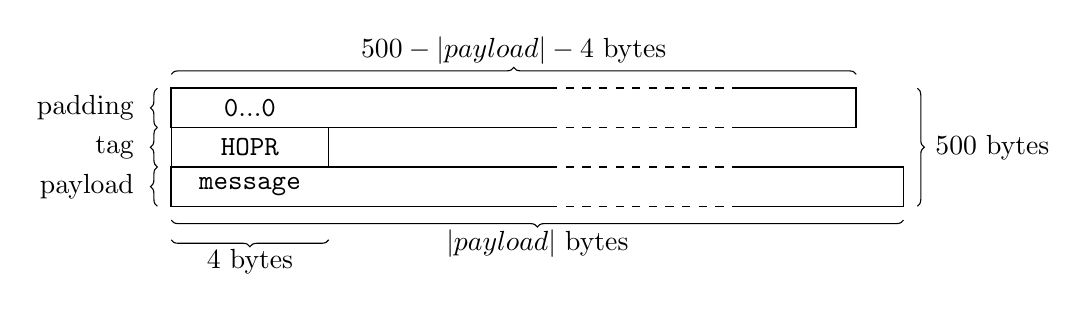
\begin{tikzpicture}
        \def\one{0.3}
        \def\lw{0.2}
        \def\middle{16*\one}
        \def\offset{8*\one}
        \def\packetLength{500}

        \def\paddingLength{29*\one}
        \def\payloadLength{31*\one}


        \draw[decoration={brace,raise=5pt},decorate] (0,0.5) -- node[above=5pt] {$\packetLength - |payload| - 4$ bytes} (\paddingLength,0.5);
        \begin{scope}
            \draw[decoration={brace,raise=5pt},decorate] (0,0) -- node[left=10pt] {padding} (0,0.5);
            \def\width{\paddingLength}
            \draw (1,0.25) node {$\mathtt{0...0}$};
            \draw [line width=\lw mm] (\middle,0.5) -- (0,0.5) --  (0,0) -- (\middle,0);
            \draw [line width=\lw mm] (\middle,0) --  (\middle+\offset, 0) [dashed];
            \draw [line width=\lw mm] (\middle,0.5) --  (\middle+\offset, 0.5) [dashed];
            \draw [line width=\lw mm] (\middle+\offset,0.5) -- (\width,0.5) --  (\width,0) -- (\middle+\offset,0);
        \end{scope}

        \begin{scope}[shift={(0,-0.5)}]
            \draw[decoration={brace,raise=5pt},decorate] (0,0) -- node[left=10pt] {tag} (0,0.5);
            \draw [draw] (0,0) rectangle (2,0.5);
            \draw (1,0.25) node {$\mathtt{HOPR}$};
        \end{scope}

        \begin{scope}[shift={(0,-1)}]
            \draw[decoration={brace,raise=5pt},decorate] (0,0) -- node[left=10pt] {payload} (0,0.5);
            \draw (1,0.25) node {$\mathtt{message}$};
            \def\width{\payloadLength}
            \draw [line width=\lw mm] (\middle,0.5) -- (0,0.5) --  (0,0) -- (\middle,0);
            \draw [line width=\lw mm] (\middle,0) --  (\middle+\offset, 0) [dashed];
            \draw [line width=\lw mm] (\middle,0.5) --  (\middle+\offset, 0.5) [dashed];
            \draw [line width=\lw mm] (\middle+\offset,0.5) -- (\width,0.5) --  (\width,0) -- (\middle+\offset,0);
        \end{scope}

        \draw[decoration={brace,raise=5pt,mirror},decorate] (0,-1.0) -- node[below=5pt] {$|payload|$ bytes} (\payloadLength,-1.0);
        \draw[decoration={brace,raise=5pt,mirror},decorate] (0,-1.25) -- node[below=5pt] {4 bytes} (2,-1.25);

        \draw[decoration={brace,raise=5pt},decorate] (\payloadLength,0.5) -- node[right=8pt] {$\packetLength$ bytes} (\payloadLength,-1.0);
    \end{tikzpicture}
    \caption{Padded message consisting of 0-padding, protocol tag $\tau$ ($\mathtt{0x484f5052}$, ASCII-encoded ``HOPR"), and payload $m$.}
\end{figure}

The sender takes the padded message and encrypts it using $\mathsf{PRP.permutate}$ with the derived subkeys in reverse order ($...,s_{i+1}^{prp}, s_i^{prp}, s_{i-1}^{prp},....$) $$\delta_i = \mathsf{PRP.permutate}_{s_i^{prp}}(\delta_{i+1})$$ where $\delta_4 = m_{pad}$ and $\delta_0$ is the ciphertext that is sent to the first relayer when using three intermediate hops.

Each node $n_i$ along the chosen path then removes one layer of encryption by setting $$\delta_{i-1} = \mathsf{PRP.inverse}_{s_i^{prp}}(\delta_i)$$ yielding $\delta_0 = m_{pad}$ in case the node is the final recipient.


\subsubsection{Shorter Paths}
\label{sec:sphinx:shorterpaths}

SPHINX packets define a maximum path length $r$, meaning $r$ intermediate mix nodes and one destination. They also allow the use of shorter paths of length $v$ with $0 \le v < r$. Despite these packets being the same size and being indistinguishable from packets with maximum path length due to their construction, it not advisable to use shorter paths since they introduce observable patterns that deviate from normal usage. By default, HOPR nodes use a path length of three and refuse to process packets with greater path lengths. 

Creating a header for shorter paths require less routing information, and thus leaves empty space in the end of $\beta$, which is filled as suggested by \cite{sphinxpaperfix} with \textit{random} data. This is necessary because the very last node, $Z$, is otherwise able to determine the path length.

\begin{figure}[H]
    \centering
    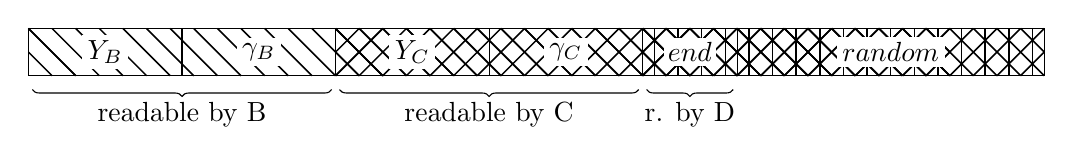
\begin{tikzpicture}
        \def\one{0.6}
        \def\scale{0.9}
        \def\nodeWidth{1.95}
        \def\endWidth{1.2}
        \def\width{3*2*\nodeWidth+\endWidth}
        \foreach \i\name in{0/B,1/C,2/D,3/Z} {
                \begin{scope}[shift={(\i*\nodeWidth*2,0)}]
                    \ifnum\i=0
                        \def\a{11.7}
                        \def\diff{11.1}
                    \fi

                    \ifnum\i=1
                        \def\a{7.8}
                        \def\diff{7.2}
                    \fi

                    \ifnum\i=2
                        \def\a{5.1}
                        \def\diff{4.5}
                    \fi

                    \def\b{\one}
                    \def\lw{0.2}

                    \ifnum\i<3
                        \foreach \x [count=\i] in{0,0.3,0.6,...,\b}{
                                \draw [line width=\lw mm](\x,0)--(0,\x) (\a-\b+\x,\b)--(\a,\x);
                            }
                        \foreach \x [count=\i] in{0,0.3,0.6,...,\diff}{
                                \draw [line width=\lw mm](\x+\b,0)--(\x,\b);
                            }

                        \ifnum\i>0
                            \foreach \x [count=\i] in{0,0.3,0.6,...,\b}{
                                    \draw [line width=\lw mm](0,\x)--(\b-\x,\b) (\a-\b+\x,0)--(\a,\b-\x);
                                }
                            \foreach \x [count=\i] in{0,0.3,0.6,...,\diff}{
                                    \draw [line width=\lw mm](\x,0)--(\b+\x,\b);
                                }
                        \fi

                        \ifnum\i>1
                            \foreach \x [count=\i] in{0.15,0.45,...,\a}{
                                    \draw [line width=\lw mm](\x,0)--(\x,\b);
                                }
                        \fi
                    \fi
                \end{scope}
                \ifnum\i=3
                    \draw (\i*2*\nodeWidth-2*\nodeWidth+\endWidth,0) rectangle (\i*2*\nodeWidth+\endWidth,\one) node [midway,fill=white,inner sep=2pt] {$random$};
                \else
                    \ifnum\i<2
                        \draw [color=white] (\i*2*\nodeWidth,0) rectangle (\i*2*\nodeWidth+\nodeWidth,\one) node [midway,color=black,fill=white,inner sep=2pt] {$Y_{\name}$};
                        \draw (\i*2*\nodeWidth,0) -- (\i*2*\nodeWidth,\one);
                        \draw [color=white] (\i*2*\nodeWidth+\nodeWidth,0) rectangle (\i*2*\nodeWidth+2*\nodeWidth,\one) node [midway,color=black,fill=white,inner sep=2pt] {$\gamma_{\name}$};
                        \draw (\i*2*\nodeWidth+\nodeWidth,0) -- (\i*2*\nodeWidth+\nodeWidth,\one);

                        \draw[decoration={brace,raise=5pt,mirror},decorate] (\nodeWidth*2*\i+0.05,0) -- (\nodeWidth*2*\i+\nodeWidth*2-0.05,0) node[midway,below=6pt] {readable by \name};
                    \else
                        \draw [color=white] (\i*2*\nodeWidth,0) rectangle (\i*2*\nodeWidth+\endWidth,\one) node [midway,color=black,fill=white,inner sep=1.5pt] {$end$};

                        \draw (\i*2*\nodeWidth,0) -- (\i*2*\nodeWidth,\one);
                        \draw (\i*2*\nodeWidth+\endWidth,0) -- (\i*2*\nodeWidth+\endWidth,\one);

                        \draw[decoration={brace,raise=5pt,mirror},decorate] (\i*2*\nodeWidth+0.05,0) -- (\i*2*\nodeWidth+\endWidth-0.05,0) node[midway,below=6pt] {r. by \name};
                    \fi
                \fi
            }

        \draw (0,0) rectangle (\width,\one);
    \end{tikzpicture}
    \caption{Node $A$ has created routing information for $B,C$ and the final recipient $D$, filling the empty part of $\beta$ with random data.}
\end{figure}

By applying the transformations seen in section \ref{sec:sphinx:shifting} through the mixnet nodes, all blindings got removed, hence the plaintext of $\beta$ becomes visible and the node is able to decide which parts of $\beta$ were not used.

\begin{figure}[H]
    \centering
    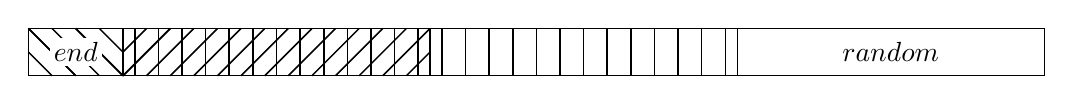
\begin{tikzpicture}
        \def\one{0.6}
        \def\scale{0.9}
        \def\nodeWidth{1.95}
        \def\endWidth{1.2}
        \def\width{3*2*\nodeWidth+\endWidth}
        \foreach \i\name in{0/B,1/C,2/D,3/Z} {
                \ifnum\i=2
                    \def\a{7.8}
                    \def\diff{7.2}
                \fi

                \ifnum\i=1
                    \def\a{3.9}
                    \def\diff{3.3}
                \fi

                \ifnum\i=0
                    \def\a{\endWidth}
                    \def\diff{0.6}
                \fi


                \def\b{0.6}
                \def\lw{0.2}

                \ifnum\i=0
                    \foreach \x [count=\i] in{0,0.3,0.6,...,\b}{
                            \draw [line width=\lw mm](\x,0)--(0,\x) (\a-\b+\x,\b)--(\a,\x);
                        }
                    \foreach \x [count=\i] in{0,0.3,0.6,...,\diff}{
                            \draw [line width=\lw mm](\x+\b,0)--(\x,\b);
                        }

                \fi
                \begin{scope}[shift={(\endWidth,0)}]
                    \ifnum\i=1
                        \foreach \x [count=\i] in{0,0.3,0.6,...,\b}{
                                \draw [line width=\lw mm](0,\x)--(\b-\x,\b) (\a-\b+\x,0)--(\a,\b-\x);
                            }
                        \foreach \x [count=\i] in{0,0.3,0.6,...,\diff}{
                                \draw [line width=\lw mm](\x,0)--(\b+\x,\b);
                            }
                    \fi

                    \ifnum\i=2
                        \foreach \x [count=\i] in{0.15,0.45,...,\a}{
                                \draw [line width=\lw mm](\x,0)--(\x,\b);
                            }
                    \fi
                \end{scope}

                \ifnum\i=3
                    \draw (\i*2*\nodeWidth-2*\nodeWidth+\endWidth,0) rectangle (\i*2*\nodeWidth+\endWidth,\one) node [midway] {$random$};
                \else
                    \ifnum\i>0
                        \draw (\i*2*\nodeWidth+\endWidth,0) -- (\i*2*\nodeWidth+\endWidth,\one);
                    \else
                        \draw [color=white] (\i*2*\nodeWidth,0) rectangle (\i*2*\nodeWidth+\endWidth,\one) node [midway,color=black,fill=white,inner sep=1.5pt] {$end$};
                        \draw (\endWidth,0) -- (\endWidth,\one);
                    \fi
                \fi
            }

        \draw (0,0) rectangle (\width,\one);
    \end{tikzpicture}
    \caption{Node $D$ receives a packet which was relayed by two intermediate nodes.}
\end{figure}



\begin{comment}
\subsection{Implementation choices}

HOPR employs the following cryptographic primitives:

\begin{itemize}
    \item \textbf{Cyclic group} HOPR's Sphinx implementation uses an elliptic curve group on the secp256k1 curve. Operations are therefore performed on the elliptic curve.

    \item \textbf{Hash function} HOPR uses the BLAKE2s hash function, a cryptographic hash function faster than SHA-2 and SHA-3, yet at least as secure as SHA-3. It produces digests of 32 bytes.

    \item \textbf{MAC} HOPR uses HMAC based on the BLAKE2s hash function.

    \item \textbf{Encryption scheme} HOPR uses the LIONESS \cite{lionesspaper} implementation, using BLAKE2s as a hash function and ChaCha20 as a stream cipher.

    \item \textbf{Padding} The original Sphinx paper uses a sequence of 0s for padding. However, this allows the last mix node in the path to infer information about the length of the path and the final destination, hence breaking one of the security properties promised by Sphinx. In order to prevent this attack, HOPR replaces the 0-padding with randomized padding for the final mix node when $v<r$. This ensures the exit node cannot identify where the padding starts and thus will not be able to determine the path length. In the case where $v=r$ there is no need to add padding as the length of the path is the maximum length, and thus no additional information is being revealed.

\end{itemize}
\end{comment}
